\documentclass[a4paper,12pt]{article}
\setcounter{secnumdepth}{2}
\newcommand{\code}[1]{{\footnotesize{{\tt #1}}}}
\usepackage{natbib}
\usepackage{color}
\usepackage{graphicx}
\usepackage{listings}
\lstset{
basicstyle=\small\ttfamily,
columns=flexible,
breaklines=true
}
\addtolength{\textwidth}{2cm} % a = -2b, where this is a and below is b
\addtolength{\hoffset}{-1cm}
\addtolength{\textheight}{2cm} % c = -d, where this is c and d is below
\addtolength{\voffset}{-2cm}
\begin{document}
\title{CASSI: Genome-Wide Interaction Analysis Software}
\date{}
\author{}
\maketitle
\newpage
\tableofcontents
\newpage
\section{Introduction}
\label{introduction}

CASSI (Contrived Acronym of Software for SNP Interactions) is a C++ program written to analyse SNP-SNP interactions, analysing a choice of SNPs from two given SNP windows (possibly from different pedigree files). Each pair of SNPs whose interaction test passes a given significance level is returned in the output file with possible extra information. The program only accepts PLINK binary files (\code{.bed}) in order to perform the calculations as efficiently as possible. 

The tests available in CASSI include those discussed by \citet{ueki:etal:12}, in particular the {\it joint effects} test. 
\begin{itemize}

\item Includes the logistic regression epistasis test for SNP-SNP interactions, but with the possibility of adding covariates to the analysis. 
\item Designed such that any number of tests may be combined to act as filters for one another, see section  section \ref{multiple-tests}. \end{itemize}

CASSI is copyright, 2012-2017 Richard Howey, GNU General Public License, version 3. 

%================== End of section "introduction"==================

\section{Installation}
\label{installation}

Download an executable file from the download$\:$page for your system and off you go, or do the following: 
\begin{enumerate}

\item Download the code from the download page. 
\item Compile it by typing something like the following: \vspace{0.35cm} \begin{lstlisting}
g++ -m64 -O3 *.cpp -o cassi

\end{lstlisting} \vspace{0.35cm}
\item Start using CASSI!\end{enumerate}

%================== End of section "installation"==================

\section{Using CASSI}
\label{using}

CASSI is executed as follows: 
\vspace{0.35cm} \begin{lstlisting}
 ./cassi [options] file.bed [file2.bed]

\end{lstlisting} \vspace{0.35cm}
or 
\vspace{0.35cm} \begin{lstlisting}
./cassi parameterfile.pf [file.bed] [file2.bed] 
\end{lstlisting} \vspace{0.35cm}
Executing CASSI either way will perform SNP interaction tests for every pair of SNPs in the \code{.bed} file (that are selected by the options). The results file will record every pair of SNPs that satisfy a given significance level together with extra information for the performed tests. A log file is also created recording the same information that is output to the screen, showing the used options and summary statistics of the data. 
\subsection{Input Files}
\label{input}

Basic usage of CASSI is to provide it with one binary PLINK format pedigree file: 
\vspace{0.35cm} \begin{lstlisting}
./cassi myfile.bed 
\end{lstlisting} \vspace{0.35cm}
This requires that the corresponding \code{.bim} and \code{.fam}, files are also available. A text PLINK pedigree file, \code{.ped}, with corresponding map file, \code{.map}, may be used to create a binary file using PLINK as follows: \vspace{0.35cm} \begin{lstlisting}
plink --noweb --file mydata --make-bed --out myfile 
\end{lstlisting} \vspace{0.35cm}

This will create the binary pedigree file, \code{myfile.bed}, map file, \code{myfile.bim}, and family file, \code{myfile.fam} required for use with CASSI. 

Two input files may also used: 
\vspace{0.35cm} \begin{lstlisting}
./cassi myfile.bed myfile2.bed

\end{lstlisting} \vspace{0.35cm}
%============ End of subsection "input"============

\subsection{Options}
\label{basic-options}

The basic options for CASSI are as follows (typing \code{./cassi} with no options will output the available options): 

{\begin{center}\begin{tabular}{ll}
Option  & Description\\
\hline
-snp1 a1 a2  & first SNP window, a1 = Start SNP number, a2 = End SNP number\\
-snp2 b1 b2  & second SNP window, b1 = Start SNP number, b2 = End SNP number\\
-i file.bed  & input file\\
-i2 file2.bed  & second (optional) input file for second SNP window\\
-o file.out  & results output file\\
-log file.log  & log file\\
-max m  & maximum number of results, to safeguard accidently outputting half a trillion results. Set to 0 for no maximum at your own risk!\\
-so  & suppress output to screen\\
-filter-all  & all statistic thresholds must be met (as ordered)\\
-filter-any  & any statistic threshold may be met\\
-gap  & gap in base pair position that SNPs need to be for case only tests. Set to 0 for no gap.\\
-mem0  & (slow) do not store SNPs in memory\\
-mem1  & (faster) store SNPs in memory, binary\\
-mem2  & (fastest) store SNPs in memory, integer\\
-rsq  & report R squared statistic between SNP pairs for cases and controls\\
-dprime  & report D' statistic between SNP pairs for cases and controls\\
\end{tabular}\end{center}}

The SNP numbers ``a1'' and ``a2'' etc. refer to the position the SNPs appears in the map file (\code{.bim}). 

For example, to use these options to analyse SNPs from SNP number 1 to SNP number 60 against SNPs from SNP number 50 to SNP number 100 using binary pedigree file \code{mydata.bed} type the following: 
\vspace{0.35cm} \begin{lstlisting}
./cassi -snp1 1 60 -snp2 50 100 mydata.bed

\end{lstlisting} \vspace{0.35cm}
This will output details of the analysis and will look something like the following: 
\vspace{0.35cm} \begin{lstlisting}
CASSI: SNP interaction analysis software, v2.00
-----------------------------------------------
Copyright 2013 Richard Howey, GNU General Public License, v3
Institute of Genetic Medicine, Newcastle University
Parameters:
Input file: mydata.bed
Output file: cassi.out
Log file: cassi.log
Start SNP of first SNP window: 1
End SNP of first SNP window: 60
Start SNP of second SNP window: 50
End SNP of second SNP window: 100
Maximum no. of results: 1000000

Data Summary Statistics:
Number of SNPs: 100
Number of subjects: 4686
Number of cases: 1748 (37.3026%)
Number of controls: 2938 (62.6974%)
Number of missing: 0

Test Statistic: Joint Effects
P-value threshold for case/control results: 0.0001
P-value threshold for case only results: 0.0001
Total SNP pairs calculated: 2994
Total SNP pair statistics passing threshold: 80

Number of SNP pairs with results: 80

Run time: less than one second

\end{lstlisting} \vspace{0.35cm}
To do the above analysis where the second SNP window is given by a different pedigree file type the following: 
\vspace{0.35cm} \begin{lstlisting}
./cassi -snp1 1 60 -snp2 50 100 mydata.bed mydata2.bed

\end{lstlisting} \vspace{0.35cm}
In addition, each different test has its own options, see the relevant sections for details. The joint effects test is used by default if no test is specified. If any tests are specified, as follows, then only these tests will be calculated. 

{\begin{center}\begin{tabular}{ll}
Option  & Description\\
\hline
-je  & do joint effects test\\
-awu  & do adjusted Wu test\\
-wz  & do Wellek Ziegler test\\
-afe  & do adjusted fast epistasis test\\
-lr  & do logistic regression test\\
\end{tabular}\end{center}}

For example, to do the adjusted Wu and adjusted fast epistasis test type: 
\vspace{0.35cm} \begin{lstlisting}
./cassi -afe -awu mydata.bed 
\end{lstlisting} \vspace{0.35cm}
{\bf Note:} Any options for individual tests must follow the option to do that test. For example: 
\vspace{0.35cm} \begin{lstlisting}
./cassi -je -je-th 1e-6 mydata.bed

\end{lstlisting} \vspace{0.35cm}
The default options for CASSI are: 

{\begin{center}\begin{tabular}{ll}
Option  & Description\\
\hline
-snp1 1 *  & All SNPs in pedigree file\\
-snp2 1 *  & All SNPs in pedigree file (or 2nd pedigree file if given)\\
-o cassi.out  & set the output file to cassi.out\\
-log cassi.log  & set the log file to cassi.log\\
-je  & use the joint effects test\\
-*-th 0.0001  & use p-value threshold of 0.0001 for any tests used\\
-max 1000000  & limit the maximum number of results to 1 million\\
-gap 1000  & SNPs need to be 1000 base pairs apart for case only tests\\
-mem2  & (fastest) store SNPs in memory, integer\\
-filter-all  & all statistic thresholds must be met (as ordered)\\
\end{tabular}\end{center}}

If the output file is set then the default log file is given by this name with the extension changed. For example, if the output file is set to \code{myresults.dat} then the default log file will be \code{myresults.log}. 

%============ End of subsection "basic-options"============

\subsection{Parameter file}
\label{parameterfile}

A parameter file, \code{.pf}, may be used with CASSI instead of writing all of the options on the command line. To use a parameter file simply type: 
\vspace{0.35cm} \begin{lstlisting}
./cassi -pf myparameters.pf 
\end{lstlisting} \vspace{0.35cm}
The parameter file should be a text file with one option written on each line. For example, to perform the analysis above the file \code{myparameters.pf} would be as follows: 
\vspace{0.35cm} \begin{lstlisting}
-snp1 1 60
-snp2 50 100
-i mydata.bed
-i2 mydata2.bed

\end{lstlisting} \vspace{0.35cm}
It is also possible to add comments to the file provided that the ``-'' character is not used, and to comment out any options by placing another character in front of any ``-''. For example, the above parameter file could be edited as follows: 
\vspace{0.35cm} \begin{lstlisting}
#This is the first SNP window
-snp1 1 60

#This is the second SNP window
-snp2 50 100

#This is the pedigree file for the first SNP window
-i mydata.bed

#This is the pedigree file for the second SNP window
-i2 mydata2.bed

#I might try this threshold later
#-th 0.00001

\end{lstlisting} \vspace{0.35cm}
%============ End of subsection "parameterfile"============

\subsection{Memory options}
\label{memory}

The default option in CASSI is to store all of the SNPs of the second window in memory as integers to allow fast calculation of the interaction tests. The first window is not stored in memory. This could be a problem if the second window has a large amount of SNPs and you do not have much memory, in which case you should consider using the \code{-mem1} option to reduce the memory usage, where the SNPs are stored in memory in binary format. 
\vspace{0.35cm} \begin{lstlisting}
./cassi -mem1 mydata.bed

\end{lstlisting} \vspace{0.35cm}
This option could be useful if you are performing tests across the whole genome and want to perform many CASSI jobs at once. The \code{-mem1} uses approximately 1/4 of the memory used by the \code{-mem2} option, but takes about 1.5 times longer to execute. If you are desperate you could use the \code{-mem0} option as follows: 
\vspace{0.35cm} \begin{lstlisting}
./cassi -mem0 mydata.bed

\end{lstlisting} \vspace{0.35cm}
This option uses very little memory by not storing the SNPs in memory but takes about 2.3 times longer to execute than the \code{-mem2} option. 

%============ End of subsection "memory"============

\subsection{$R^2$ and D'}
\label{rsq}

It is possible to output the $R^2\ $and/or the D' values between SNP pairs for the cases and controls with the \code{-rsq} and \code{-dprime} options respectively. For example, to output both of these: 
\vspace{0.35cm} \begin{lstlisting}
./cassi -je -rsq -dprime mydata.bed

\end{lstlisting} \vspace{0.35cm}
This will output the $R^2\ $values for the cases and controls, given by columns CASE\_RSQ$\:$and CTRL\_RSQ$\:$respectively. The D' values for the cases and controls are given by columns CASE\_DPRIME$\:$and CTRL\_DPRIME$\:$respectively. The output will look something like the following: 
\vspace{0.35cm} \begin{lstlisting}
SNP1 CHR1 ID1 BP1 SNP2 CHR2 ID2 BP2 JE_CASE_LOG_OR JE_CASE_SE JE_CTRL_LOG_OR JE_CTRL_SE JE_CC_CHISQ JE_CC_P JE_CC_ALT JE_CO_CHISQ JE_CO_P JE_CO_ALT 
   CASE_RSQ CTRL_RSQ CASE_DPRIME CTRL_DPRIME
1 1 rs3825035 207140 11 1 rs6598035 242318 0.77282 0.148039 0.706996 0.154282 0.0947709 0.758197 N 27.2524 1.78554e-07 N 0.0240119 0.0251859 0.265702 0.233982
3 1 rs1027430 214393 24 1 rs7394810 356710 -0.617103 0.145369 -0.909585 0.141284 2.08175 0.149069 N 18.0209 2.18499e-05 N 0.0172226 0.0397905 0.244953 0.338341
16 1 rs1227455 252234 24 1 rs7394810 356710 0.668421 0.140027 0.517802 0.141032 0.574359 0.448532 N 22.7864 1.81045e-06 N 0.0225344 0.013668 0.225165 0.181016
16 1 rs1227455 252234 69 1 rs1126386 1034938 -0.680131 0.150314 -0.559377 0.150018 0.323315 0.569622 N 20.4732 6.04708e-06 N 0.0201808 0.0135523 0.285269 0.238255
19 1 rs4718635 273928 42 1 rs1090209 723609 0.524665 0.129452 0.135148 0.123059 4.75603 0.0291958 N 16.4266 5.05695e-05 N 0.0172832 0.00111035 0.146305 0.0369723
...

\end{lstlisting} \vspace{0.35cm}
If no test statistic is given to CASSI $R^2\ $and/or D' values are calculated and output. To output these extras values together with a test statistic meeting a threshold, the \code{-rsq} and \code{-dprime} options should be listed {\it after} the test statistic option, otherwise these will be calculated unnecessarily for test statistics not meeting the threshold. 

%============ End of subsection "rsq"============


%================== End of section "using"==================

\section{Joint Effects}
\label{joint-effects}

For full details of the joints effects test and the accompanying notation please refer to the manuscript by \citet{ueki:etal:12}. 
\subsection{Options}
\label{je-options}

The options that are specific to the joint effects test are: 

{\begin{center}\begin{tabular}{ll}
Option  & Description\\
\hline
-je  & perform the joint effects test\\
-je-thcc t  & p-value threshold for case/control test\\
-je-thco t  & p-value threshold for case only test\\
-je-th t  & p-value threshold for either test\\
-je-cc-only  & perform the case/control test only\\
-je-co-only  & perform the case only test only\\
-je-cellmin m  & minimum cell count required in each cell to perform test\\
-je-so  & suppress results of test\\
\end{tabular}\end{center}}

CASSI performs both the case only test and case/control test for each pair of tested SNPs by default. The results of the test are recorded for the pair of SNPs if {\it either} p-value threshold is met. Both thresholds may be set simultaneously by using the \code{-je-th} option. The default value for both thresholds is 0.0001. 

To avoid issues with insufficient data, a minimum number cell count is required (where cells are given by the genotype combinations, 9 for cases and 9 for controls). The default number is set to 5, but can be changed with the \code{-je-mincell} option. Setting the cell count minimum to 0 obviously gives no minimum. If there is no cell minimum and any cells are 0 then all any cells will have 0.5 added. 

For other basic options see  section \ref{basic-options}. 

%============ End of subsection "je-options"============

\subsection{Output File}
\label{je-output}

The output file from running a joint effects SNP interaction analysis using CASSI will look something like the following: 
\vspace{0.35cm} \begin{lstlisting}
SNP1 CHR1 ID1 BP1 SNP2 CHR2 ID2 BP2 JE_CASE_LOG_OR JE_CASE_SE JE_CTRL_LOG_OR JE_CTRL_SE JE_CC_CHISQ JE_CC_P JE_ALT_CC JE_CO_CHISQ JE_CO_P JE_ALT_CO
4 1 rs5367015 220368 558 1 rs7129551 4544990 6.34341 0.632507 3.65647 0.597288 2.00984 0.156282 N 16.0982 6.01412e-05 N
5 1 rs12363280 221980 506 1 rs1102289 4422547 4.1916 1.04833 4.15869 1.04265 0.00334286 0.953894 N 19.3086 1.11203e-05 N
5 1 rs12363280 221980 512 1 rs1083109 4447884 5.17158 0.820119 4.93334 0.742762 0.467668 0.494062 N 17.9887 2.22222e-05 N
5 1 rs12363280 221980 526 1 rs1500597 4483159 4.1916 1.04833 4.15869 1.04265 0.00334286 0.953894 N 19.3086 1.11203e-05 N
5 1 rs12363280 221980 551 1 rs1103294 4534498 4.63789 0.970636 4.36155 0.95259 0.0916524 0.762087 N 20.2653 6.74113e-06 N
... 
 
\end{lstlisting} \vspace{0.35cm}
The first line is a header labelling the columns of the results file. The SNP details for the pair of SNPs are given firstly followed by values calculated from the joint effects tests. Results are given for both the case only test and for the case/control test regardless of which p-value was significant enough to record the pair of SNPs. The case only test assumes that the two SNPs are in linkage equilibrium in the general population, so care must be taken in interpreting results with SNPs that are near one another. Therefore, SNPs that are too close, as definded by the \code{-gap} option, are not tested. See \citet{ueki:etal:12}. 

{\bf JE\_CASE\_LOG\_OR} is the log odds ratio for association in the cases and is given by $\tilde{\lambda}_A$. If the alternative test is used this is given by $\tilde{\mu}_A$. 

{\bf JE\_CASE\_SE} is the standard error of $\tilde{\lambda}_A$ and is given by the square root of $\tilde{\nu}_A$. If the alternative test is used the standard error for $\tilde{\mu}_A$ is recorded, given by the square root of $\tilde{\nu}_{\mu_A}$. 

{\bf JE\_CTRL\_LOG\_OR} is the log odds ratio for association in the controls and is given by $\tilde{\lambda}_N$. If the alternative test is used this is given by $\tilde{\mu}_N$. 

{\bf JE\_CTRL\_SE} is the standard error of $\tilde{\lambda}_N$ and is given by the square root of $\tilde{\nu}_N$. If the alternative test is used the standard error for $\tilde{\mu}_N$ is recorded, given by the square root of $\tilde{\nu}_{\mu_N}$. 

{\bf JE\_CC\_CHISQ} is the $\chi^2$ test statistic with one degree of freedom for the case/control test. 

{\bf JE\_CC\_P} is the corresponding p-value for the case/control test. 

{\bf JE\_CC\_ALT} whether or not the alternative statistic was used for the case/control test. 

{\bf JE\_CO\_CHISQ} is the $\chi^2$ test statistic with one degree of freedom for the case only test. 

{\bf JE\_CO\_P} is the corresponding p-value for the case only test. 

{\bf JE\_CO\_ALT} whether or not the alternative statistic was used for the case only test. 

%============ End of subsection "je-output"============


%================== End of section "joint-effects"==================

\section{Adjusted Wu}
\label{adjusted-wu}

The adjusted Wu test is described by \citet{ueki:etal:12} and is a corrected version of a test proposed by \citet{Wu:etal:2010} . The test is based on the 4 estimated haplotype frequencies between the two SNPs that are being tested (calculated using the EM algorithm in CASSI). 
\subsection{Options}
\label{awu-options}

The options that are specific to the adjusted Wu test are: 

{\begin{center}\begin{tabular}{ll}
Option  & Description\\
\hline
-awu  & perform the adjusted Wu test\\
-awu-thcc t  & p-value threshold for case/control test\\
-awu-thco t  & p-value threshold for case only test\\
-awu-th t  & p-value threshold for either test\\
-awu-cc-only  & perform the case/control test only\\
-awu-co-only  & perform the case only test only\\
-awu-so  & suppress results of test\\
\end{tabular}\end{center}}

CASSI performs both the case only test and case/control test for each pair of tested SNPs by default. SNPs that are too close for the case only test, as definded by the \code{-gap} option, are not tested. The results of the test are recorded for the pair of SNPs if {\it either} p-value threshold is met. Both thresholds may be set simultaneously by using the \code{-awu-th} option. The default value for both thresholds is 0.0001. 

For other basic options see  section \ref{basic-options}. 

%============ End of subsection "awu-options"============

\subsection{Output File}
\label{awu-output}

The output file from running an adjusted Wu SNP interaction analysis using CASSI will look something like the following: 
\vspace{0.35cm} \begin{lstlisting}
SNP1 CHR1 ID1 BP1 SNP2 CHR2 ID2 BP2 AWU_CASE_LOG_OR AWU_CASE_SE AWU_CTRL_LOG_OR AWU_CTRL_LOG_SE AWU_CC_CHISQ AWU_CC_P AWU_CO_CHISQ AWU_CO_P
1306 1 rs285785 6939568 542 1 rs2657173 4519034 0.663321 0.154558 0.247584 0.158968 3.51587 0.0607836 18.4189 1.77292e-05
1306 1 rs285785 6939568 544 1 rs26414414 4519523 0.671198 0.154619 0.208327 0.15861 4.36672 0.0366475 18.844 1.41854e-05
1349 1 rs150628 7172817 572 1 rs22312963 4581596 -0.734064 0.180251 -0.00671448 0.178903 8.20253 0.0041832 16.5849 4.65207e-05
1352 1 rs185794 7190018 639 1 rs794332 4807931 -0.604667 0.13482 -0.299917 0.133023 2.58902 0.107607 20.1152 7.29157e-06
...

\end{lstlisting} \vspace{0.35cm}
The first line is a header labelling the columns of the results file. The SNP details for the pair of SNPs are given firstly followed by values calculated from the joint effects tests. Results are given for both the case only test and for the case/control test regardless of which p-value was significant enough to record the pair of SNPs. The case only test assumes that the two SNPs are in linkage equilibrium in the general population, so care must be taken in interpreting results with SNPs that are near one another. See \citet{ueki:etal:12}. 

{\bf AWU\_CASE\_LOG\_OR} is the log odds ratio for association in the cases. 

{\bf AWU\_CASE\_SE} is the standard error of AWU\_CASE\_LOG\_OR.

{\bf AWU\_CTRL\_LOG\_OR} is the log odds ratio for association in the controls. 

{\bf AWU\_CTRL\_SE} is the standard error of AWU\_CTRL\_LOG\_OR.

{\bf AWU\_CC\_CHISQ} is the $\chi^2$ test statistic with one degree of freedom for the case/control test. 

{\bf AWU\_CC\_P} is the corresponding p-value for the case/control test. 

{\bf AWU\_CO\_CHISQ} is the $\chi^2$ test statistic with one degree of freedom for the case only test. 

{\bf AWU\_CO\_P} is the corresponding p-value for the case only test. 

%============ End of subsection "awu-output"============


%================== End of section "adjusted-wu"==================

\section{Adjusted Fast Epistasis}
\label{adjusted-fast-epistasis}

The adjusted fast epistasis test is a corrected version of the fast epistasistest as implemented in PLINK \citet{purcell:etal:07}, and is described by \citet{ueki:etal:12}. Despite requiring some extra calculation the adjusted fast epistasis test in CASSI runs faster than the fast epistasis test in PLINK, see  section \ref{run-times} for details. 
\subsection{Options}
\label{afe-options}

The options that are specific to the adjusted fast epistasis test are: 

{\begin{center}\begin{tabular}{ll}
Option  & Description\\
\hline
-afe  & perform the adjusted fast epistasis test\\
-afe-thcc t  & p-value threshold for case/control test\\
-afe-thco t  & p-value threshold for case only test\\
-afe-th t  & p-value threshold for either test\\
-afe-cc-only  & perform the case/control test only\\
-afe-co-only  & perform the case only test only\\
-afe-so  & suppress results of test\\
\end{tabular}\end{center}}

CASSI performs both the case only test and case/control test for each pair of tested SNPs by default. SNPs that are too close for the case only test, as definded by the \code{-gap} option, are not tested. The results of the test are recorded for the pair of SNPs if {\it either} p-value threshold is met. Both thresholds may be set simultaneously by using the \code{-afe-th} option. The default value for both thresholds is 0.0001. 

For other basic options see  section \ref{basic-options}. 

%============ End of subsection "afe-options"============

\subsection{Output File}
\label{afe-output}

The output file from running an adjusted fast epistasis SNP interaction analysis using CASSI will look something like the following: 
\vspace{0.35cm} \begin{lstlisting}
SNP1 CHR1 ID1 BP1 SNP2 CHR2 ID2 BP2 AFE_CASE_LOG_OR AFE_CASE_SE AFE_CTRL_LOG_OR AFE_CTRL_SE AFE_CC_CHISQ AFE_CC_P AFE_CO_CHISQ AFE_CO_P
2 1 rs1103289 207421 5 1 rs1233280 221980 6.15411 1.08027 5.9423 1.0608 0.0195714 0.888741 32.454 1.22046e-08
2 1 rs1103289 207421 6 1 rs498039 222598 6.7911 1.18655 6.7911 1.18655 0 1 32.7571 1.04422e-08
2 1 rs1103289 207421 12 1 rs65417 242851 4.28441 1.00451 4.80692 1.01244 0.134221 0.714096 18.1915 1.99764e-05
2 1 rs1103289 207421 25 1 rs1246136 361265 6.7911 1.18655 6.7911 1.18655 0 1 32.7571 1.04422e-08
2 1 rs1103289 207421 46 1 rs1246300 739776 6.7911 1.18655 6.7911 1.18655 0 1 32.7571 1.04422e-08
...

\end{lstlisting} \vspace{0.35cm}
The first line is a header labelling the columns of the results file. The SNP details for the pair of SNPs are given firstly followed by values calculated from the joint effects tests. Results are given for both the case only test and for the case/control test regardless of which p-value was significant enough to record the pair of SNPs. The case only test assumes that the two SNPs are in linkage equilibrium in the general population, so care must be taken in interpreting results with SNPs that are near one another. See \citet{ueki:etal:12}. 

{\bf AFE\_CASE\_LOG\_OR} is the log odds ratio for association in the cases. 

{\bf AFE\_CASE\_SE} the standard error of AFE\_CASE\_LOG\_OR.

{\bf AFE\_CTRL\_LOG\_OR} is the log odds ratio for association in the controls. 

{\bf AFE\_CTRL\_SE} is the standard error of AFE\_CTRL\_LOG\_OR.

{\bf AFE\_CC\_CHISQ} is the $\chi^2$ test statistic with one degree of freedom for the case/control test. 

{\bf AFE\_CC\_P} is the corresponding p-value for the case/control test. 

{\bf AFE\_CO\_CHISQ} is the $\chi^2$ test statistic with one degree of freedom for the case only test. 

{\bf AFE\_CO\_P} is the corresponding p-value for the case only test. 

%============ End of subsection "afe-output"============


%================== End of section "adjusted-fast-epistasis"==================

\section{Wellek Ziegler}
\label{wellek-ziegler}

The Wellek Ziegler test, as defined by \citet{ueki:etal:12}, is based on the Pearson product-moment correlation coefficient, {\it r}, and is inspired by tests proposed by \citet{wellek:ziegler:09}. 
\subsection{Options}
\label{wz-options}

The options that are specific to the Wellek Ziegler test are: 

{\begin{center}\begin{tabular}{ll}
Option  & Description\\
\hline
-wz  & perform the Wellek Ziegler test\\
-wz-thcc t  & p-value threshold for case/control test\\
-wz-thco t  & p-value threshold for case only test\\
-wz-th t  & p-value threshold for either test\\
-wz-cc-only  & perform the case/control test only\\
-wz-co-only  & perform the case only test only\\
-wz-so  & suppress results of test\\
\end{tabular}\end{center}}

CASSI performs both the case only test and case/control test for each pair of tested SNPs by default. SNPs that are too close for the case only test, as definded by the \code{-gap} option, are not tested. The results of the test are recorded for the pair of SNPs if {\it either} p-value threshold is met. Both thresholds may be set simultaneously by using the \code{-wz-th} option. The default value for both thresholds is 0.0001. 

For other basic options see  section \ref{basic-options}. 

%============ End of subsection "wz-options"============

\subsection{Output File}
\label{wz-output}

The output file from running a Wellek Ziegler SNP interaction analysis using CASSI will look something like the following: 
\vspace{0.35cm} \begin{lstlisting}
SNP1 CHR1 ID1 BP1 SNP2 CHR2 ID2 BP2 WZ_CASE_R WZ_CASE_VAR WZ_CTRL_R WZ_CTRL_VAR WZ_CC_CHISQ WZ_CC_P WZ_CO_CHISQ WZ_CO_P
117 0 rs1076866 1588987 934 0 rs4547126 5543590 -0.102088 0.00080134 0.0818521 0.0011718 17.1473 3.45901e-05 13.0057 0.000310544
174 0 rs7343521 2112789 948 0 rs1083841 5601579 0.131803 0.00111305 0.0109372 0.0010405 6.78342 0.00920083 15.6074 7.79475e-05
174 0 rs7343521 2112789 949 0 rs1227893 5603609 0.138261 0.00112451 0.0221176 0.00105799 6.18069 0.0129152 16.9996 3.73873e-05
177 0 rs3741208 2126350 918 0 rs7934354 5522482 -0.121458 0.000872938 0.0162084 0.00101684 10.0287 0.00154121 16.8992 3.94175e-05
198 0 rs1228842 2352598 899 0 rs1727848 5490415 -0.0628705 0.000910977 0.117571 0.00102275 16.8375 4.07198e-05 4.33896 0.0372496
...

\end{lstlisting} \vspace{0.35cm}
The first line is a header labelling the columns of the results file. The SNP details for the pair of SNPs are given firstly followed by values calculated from the Wellek Ziegler tests. Results are given for both the case only test and for the case/control test regardless of which p-value was significant enough to record the pair of SNPs. The case only test assumes that the two SNPs are in linkage equilibrium in the general population, so care must be taken in interpreting results with SNPs that are near one another. See \citet{ueki:etal:12}. 

{\bf WZ\_CASE\_R} is the Pearson product-moment correlation coefficient for association in the cases. 

{\bf WZ\_CASE\_VARR} is the variance of WZ\_CASE\_R.

{\bf WZ\_CTRL\_R} is the Pearson product-moment correlation coefficient for association in the controls. 

{\bf WZ\_CTRL\_VARR} is the variance of WZ\_CTRL\_R.

{\bf WZ\_CC\_CHISQ} is the $\chi^2$ test statistic with one degree of freedom for the case/control test. 

{\bf WZ\_CC\_P} is the corresponding p-value for the case/control test. 

{\bf WZ\_CO\_CHISQ} is the $\chi^2$ test statistic with one degree of freedom for the case only test. 

{\bf WZ\_CO\_P} is the corresponding p-value for the case only test. 

%============ End of subsection "wz-output"============


%================== End of section "wellek-ziegler"==================

\section{Logistic Regression}
\label{logistic-regression}

The logistic regression test in CASSI is essentially the same as the epistasistest as implemented in PLINK \citet{purcell:etal:07}. The difference being that CASSI uses the likelihood ratio test between logistic regression models with and without an interaction term. Furthermore, CASSI has the added bonuses of running much faster (see  section \ref{run-times}) and being able to incorporate covariates into the analysis, as well as being able to use any other test in CASSI as a screening step. 
\subsection{Options}
\label{lr-options}

The options that are specific to the logistic regression test are: 

{\begin{center}\begin{tabular}{ll}
Option  & Description\\
\hline
-lr  & perform the logistic regression test\\
-lr-th t  & p-value threshold for the logistic regression test\\
-lr-so  & suppress results of test\\
-lr-covar covariates.dat  & set covariate file, covariates.dat\\
-lr-covar-number nums  & only use covariates given by the numbers, nums\\
-lr-covar-name na  & only use covariates given by the names, na\\
-lr-covar-miss x  & set missing covariate value, x\\
\end{tabular}\end{center}}

The default p-value threshold is 0.0001 and the default missing covariate value is -9. 

For other basic options see  section \ref{basic-options}. 

%============ End of subsection "lr-options"============

\subsection{Output File}
\label{lr-output}

The output file from running a logistic regression epistatis analysis using CASSI will look something like the following: 
\vspace{0.35cm} \begin{lstlisting}
SNP1 CHR1 ID1 BP1 SNP2 CHR2 ID2 BP2 LR_LOG_OR LR_SE LR_CHISQ LR_P
541 1 rs2657274 4518966 783 1 rs7931851 5254756 0.37203 0.0946377 15.4536 8.45579e-05
542 1 rs2657273 4519034 783 1 rs7931851 5254756 0.422308 0.0973076 18.8349 1.42531e-05
544 1 rs2641314 4519523 783 1 rs7931851 5254756 0.423179 0.0963309 19.2982 1.11809e-05
556 1 rs1505116 4535285 637 1 rs1732891 4800616 -1.41948 0.364753 15.1446 9.95837e-05
609 1 rs7117459 4708712 621 1 rs1278492 4750695 17.9602 4.54453 15.6186 7.74883e-05
...

\end{lstlisting} \vspace{0.35cm}
The first line is a header labelling the columns of the results file. The SNP details for the pair of SNPs are given firstly followed by values calculated from the logistic regression test. 

{\bf LR\_LOG\_OR} is the log odds ratio for interaction. 

{\bf LR\_SE} is the standard error of LR\_LOG\_OR$\:$(given by assuming LR\_LOG\_OR$\:$squared divided by its variance approximates the $\chi^2$ test statistic). 

{\bf LR\_CHISQ} is the $\chi^2$ test statistic with one degree of freedom. 

{\bf LR\_P} is the corresponding p-value. 

%============ End of subsection "lr-output"============

\subsection{Covariates}
\label{covariates}

It is possible to perform the logistic regression test with a set of covariates. To do this use the \code{-lr-covar} option. For example: 
\vspace{0.35cm} \begin{lstlisting}
./cassi -lr -lr-covar covariates.dat mydata.bed

\end{lstlisting} \vspace{0.35cm}
Unfortunately, the logistic regression test with covariates is very s-s-s-s-slow (see  section \ref{run-times}), so a large analysis is not advisable. However, this is not a problem as any other test in CASSI can be used as a screening step before performing logistic regression with covariates. See  section \ref{multiple-tests} for details. 

The format of the covariate file is the same as PLINK covariate files. That is, a text file where the first column is the pedigree ID, the second column is the individual ID and the remaining columns are the covariate values, where a value of -9 denotes a missing value (this may be changed with the \code{-lr-covar-miss} option). For example, a covariate file with 3 covariates may look as follows: 
\vspace{0.35cm} \begin{lstlisting}
PEDID ID SMOKE ALCOHOL EX
WXA_T123 QWA_T120 0.0032 0.0033 0.0207
WXA_T123 QWA_T121 -0.0019 0.022 0.0247
WXA_T124 QWA_T987 0.0104 0.0096 -0.0154
...

\end{lstlisting} \vspace{0.35cm}
The header line may be present or not. The covariates may be chosen with the header names as follows: 
\vspace{0.35cm} \begin{lstlisting}
./cassi -lr -lr-covar covariates.dat -lr-covar-name ALCOHOL,EX -o myresults.dat mydata.bed

\end{lstlisting} \vspace{0.35cm}
or 
\vspace{0.35cm} \begin{lstlisting}
./cassi -lr -lr-covar covariates.dat -lr-covar-name ALCOHOL-EX -o myresults.dat mydata.bed

\end{lstlisting} \vspace{0.35cm}
to include all covariates between and including these two. Note that no spaces should be used between the chosen covariate values. The covariates may also be chosen by their numbers. So the above may be written: 
\vspace{0.35cm} \begin{lstlisting}
./cassi -lr -lr-covar covariates.dat -lr-covar-name 2,3 -o myresults.dat mydata.bed

\end{lstlisting} \vspace{0.35cm}
or 
\vspace{0.35cm} \begin{lstlisting}
./cassi -lr -lr-covar covariates.dat -lr-covar-name 2-3 -o myresults.dat mydata.bed

\end{lstlisting} \vspace{0.35cm}
The output file from running a logistic regression analysis with covariates will look something like the following: 
\vspace{0.35cm} \begin{lstlisting}
SNP1 CHR1 ID1 BP1 SNP2 CHR2 ID2 BP2 LR_COVAR_LOG_OR LR_COVAR_SE LR_COVAR_CHISQ LR_COVAR_P
135 1 rs1627458 1633498 297 1 rs451041 3017301 0.381645 0.091521 17.3892 3.04559e-05
135 1 rs1627458 1633498 299 1 rs711857 3024682 0.388182 0.0932027 17.3466 3.11453e-05
143 1 rs1627507 1673325 216 1 rs794012 2549107 2.60804 0.665518 15.3571 8.89863e-05
166 1 rs2107425 1977651 203 1 rs108134 2459062 0.574884 0.146822 15.3313 9.02099e-05
200 1 rs7570914 2397565 371 1 rs267216 3648600 0.726192 0.184818 15.4388 8.52196e-05
...

\end{lstlisting} \vspace{0.35cm}
That is, it is the same as before but with a different header, which is useful when performing logistic regression with and without covariates. 

%============ End of subsection "covariates"============


%================== End of section "logistic-regression"==================

\section{Linear Regression}
\label{linear-regression}

If the phenotype of the individuals is quantitative rather than case-control status then it is possible to use CASSI to test for epistasis using linear regression. This is done by fitting two linear regression models, one with an interaction term and one without, and these models are then compared using an F-test with their residual sum of squares. As with logistic regression it is also possible to incorporate covariates into any analysis. When covariates are included, linear regression is faster (see  section \ref{run-times}) than logistic regression and may be useful as a screening step, see  section \ref{screening}. 
\subsection{Options}
\label{lin-options}

The options that are specific to the linear regression test are: 

{\begin{center}\begin{tabular}{ll}
Option  & Description\\
\hline
-lin  & perform the linear regression test\\
-lin-th t  & p-value threshold for the linear regression test\\
-lin-so  & suppress results of test\\
-lin-covar covariates.dat  & set covariate file, covariates.dat\\
-lin-covar-number nums  & only use covariates given by the numbers, nums\\
-lin-covar-name na  & only use covariates given by the names, na\\
-lin-covar-miss x  & set missing covariate value, x\\
\end{tabular}\end{center}}

The default p-value threshold is 0.0001 and the default missing covariate value is -9. 

For other basic options see  section \ref{basic-options}. 

%============ End of subsection "lin-options"============

\subsection{Output File}
\label{lin-output}

The output file from running a linear regression epistatis analysis using CASSI will look something like the following: 
\vspace{0.35cm} \begin{lstlisting}
SNP1 CHR1 ID1 BP1 SNP2 CHR2 ID2 BP2 LIN_BETA LIN_BETA_SE LIN_FSTAT LIN_P
541 1 rs2657134 4518966 783 1 rs7931361 5254756 0.0919379 0.0233854 15.4561 8.73237e-05
542 1 rs2657163 4519034 783 1 rs7931361 5254756 0.104137 0.0239852 18.8505 1.48449e-05
544 1 rs2641444 4519523 783 1 rs7931361 5254756 0.104289 0.0237317 19.3118 1.16842e-05
639 1 rs7934332 4807931 651 1 rs1103368 4837468 0.130456 0.030614 18.1587 2.12699e-05
642 1 rs1103114 4809648 651 1 rs1103368 4837468 0.130489 0.0308339 17.9098 2.42124e-05
... 

\end{lstlisting} \vspace{0.35cm}
The first line is a header labelling the columns of the results file. The SNP details for the pair of SNPs are given firstly followed by values calculated from the linear regression test. 

{\bf LIN\_BETA} interaction regression coefficient. 

{\bf LIN\_BETA\_SE} is the standard error of the interaction regression coefficient. 

{\bf LIN\_FSTAT} is the F-test statistic. 

{\bf LIN\_P} is the corresponding p-value. 

%============ End of subsection "lin-output"============

\subsection{Covariates}
\label{lin-covariates}

It is possible to perform linear regression with a set of covariates. To do this use the \code{-lin-covar} option. For example: 
\vspace{0.35cm} \begin{lstlisting}
./cassi -lin -lin-covar covariates.dat mydata.bed

\end{lstlisting} \vspace{0.35cm}
The format of the covariate file is the same as for logistic regression, see  section \ref{covariates}. 

The output file from running a linear regression analysis with covariates will look something like the following: 
\vspace{0.35cm} \begin{lstlisting}
SNP1 CHR1 ID1 BP1 SNP2 CHR2 ID2 BP2 LIN_COVAR_BETA LIN_COVAR_BETA_SE LIN_COVAR_FSTAT LIN_COVAR_P
541 1 rs2647164 4518966 783 1 rs7931851 5253756 0.0927018 0.0234313 15.6524 7.87797e-05
542 1 rs2647163 4519034 783 1 rs7931851 5253756 0.106082 0.0240464 19.4619 1.08102e-05
544 1 rs2641444 4519523 783 1 rs7931851 5253756 0.1055 0.0237654 19.7067 9.52224e-06
639 1 rs7934322 4807931 651 1 rs1103368 4837461 0.129999 0.0306687 17.9675 2.34979e-05
642 1 rs1103114 4809648 651 1 rs1103368 4837461 0.129712 0.0308939 17.6284 2.80373e-05
...

\end{lstlisting} \vspace{0.35cm}
That is, it is the same as before but with a different header, which is useful when performing linear regression with and without covariates. 

%============ End of subsection "lin-covariates"============


%================== End of section "linear-regression"==================

\section{Filtering Multiple Tests}
\label{multiple-tests}

It is possible to simultaneously calculate more than one test in CASSI and to use the tests as screening steps if desired. 
\subsection{Screening Tests}
\label{screening}

To use one test to screen for another one is easy with CASSI. There will be quite few options to give to CASSI, so the easiest thing to do will is to write a parameter file. For example, save the following as \code{myparas.pf} 
\vspace{0.35cm} \begin{lstlisting}
#Set up input and output files
-i chromosome1.bed
-o myresults.dat

#Do logistic regression test as a screening step
-lr
-lr-th 0.001

#Do logistic regression test with 4 covariates
-lr
-lr-th 0.0001
-lr-covar covariates.dat

\end{lstlisting} \vspace{0.35cm}
and then run CASSI as follows: 
\vspace{0.35cm} \begin{lstlisting}
./cassi -pf myparas.pf

\end{lstlisting} \vspace{0.35cm}
The above example uses logistic regression with a p-value threshold of 0.001 as a screening step for logistic regression with 4 covariates. The tests are ran in the order they appear in the parameter file or the command line. The output will look something like: 
\vspace{0.35cm} \begin{lstlisting}
SNP1 CHR1 ID1 BP1 SNP2 CHR2 ID2 BP2 LR_LOG_OR LR_CHISQ LR_P LR_COVAR_LOG_OR LR_COVAR_CHISQ LR_COVAR_P
1 1 rs3825075 207140 1022 1 rs11039351 5842422 0.729394 15.2732 9.30269e-05 0.730193 15.2866 9.23706e-05
1 1 rs3825075 207140 1188 1 rs12794064 6674133 0.753422 14.7342 0.00012378 0.766574 15.2141 9.59825e-05
1 1 rs3825075 207140 1355 1 rs71037479 7211075 -0.56288 18.998 1.30857e-05 -0.567815 19.282 1.12763e-05
13 1 rs659804 244010 2703 1 rs10831905 12733043 2.43204 17.5586 2.78587e-05 2.45784 17.9211 2.30255e-05
13 1 rs659804 244010 2717 1 rs10500759 12779164 2.05542 15.5899 7.86735e-05 2.07359 15.9522 6.49639e-05

\end{lstlisting} \vspace{0.35cm}
My test data of 3000 SNPs took about 7 minutes to calculate the 4,498,500 SNP pair tests, compared to about 22 hours without the screening step - and resulted in the same results. Nice. To speed things up further we can add another screening stage using the adjusted fast epistasis test: 
\vspace{0.35cm} \begin{lstlisting}
#Set up input and output files
-i chromosome1.bed
-o myresults.dat

#Do the adjusted fast epistasis test as a screening step
-afe
-afe-th 0.2

#Do logistic regression test as a screening step
-lr
-lr-th 0.001

#Do logistic regression test with 4 covariates
-lr
-lr-th 0.0001
-lr-covar covariates.dat

\end{lstlisting} \vspace{0.35cm}
The runtime for the above analysis took about 5 and a half minutes to analysis the same data set and resulted in the same results. Obviously, the smaller the p-value threshold that is set for a screening step the quicker the analysis will run, but setting it too small may result in missing some significant test results in the last test. A comparison of the runtimes of each test are shown in  section \ref{run-times} which may act as a guide as to which order to run the tests. The log file will show how many tests passed at each step and the log file for the above analysis looked like this: 
\vspace{0.35cm} \begin{lstlisting}
CASSI: SNP interaction analysis software, v2.00
-----------------------------------------------
Copyright 2013 Richard Howey, GNU General Public License, v3
Institute of Genetic Medicine, Newcastle University

Parameters:
Input file: chromosome1.bed
Output file: myresults.dat
Log file: myresults.log
Start SNP of first SNP window: 1
End SNP of first window is the last SNP
Start SNP of second SNP window: 1
End SNP of second window is the last SNP
Maximum no. of results: 1000000
Filter: all statistic thresholds must pass

Data Summary Statistics:
Number of SNPs: 3000
Number of subjects: 2000
Number of cases: 1000 (50%)
Number of controls: 1000 (50%)
Number of missing: 0

Test Statistic: Adjusted Fast Epistasis
P-value threshold for case/control results: 0.2
P-value threshold for case only results: 0.2
Total SNP pairs calculated: 4498500
Total SNP pair statistics passing threshold: 1753516

Test Statistic: Logistic Regression
P-value threshold for case/control results: 0.001
Total SNP pairs calculated: 1753516
Total SNP pair statistics passing threshold: 4055

Test Statistic: Logistic Regression
Covariate file: covariates.dat (with missing value -9)
P-value threshold for case/control results: 0.0001
Total SNP pairs calculated: 4055
Total SNP pair statistics passing threshold: 461

Number of SNP pairs with results: 461

Run time: 5 minutes and 24 seconds

\end{lstlisting} \vspace{0.35cm}
It can be seen that the first step reduces the number of tests to be performed by logistic regression by about 60 percent. The final step only tests about 0.09 percent of the original SNP pairs, speeding up the analysis considerably. 

%============ End of subsection "screening"============

\subsection{Calculating All Tests}
\label{calculate-all}

It is also possible to calculate a number of tests and report results whenever any of the p-value thresholds are passed. This is done with the \code{-filter-any} option. For example, using the following parameter file: 
\vspace{0.35cm} \begin{lstlisting}
#Set up input and output files
-i chromosome1.bed
-o myresults.dat

#Set filter to allow any p-value threshold to be passed
-filter-any

#Do the adjusted fast epistasis test
-afe
-afe-th 1e-4

#Do Wellek Ziegler test
-wz
-wz-th 1e-5

\end{lstlisting} \vspace{0.35cm}
will produce results where either the adjusted fast epistasis test gives a p-value less than 0.0001 or the Wellek Ziegler test gives a p-value less than 0.00001. 

Every test will be evaluated when using the \code{-filter-any} option so the order of the tests in this case is not so important. 

%============ End of subsection "calculate-all"============

\subsection{Runtimes}
\label{run-times}

Figure  \ref{runtimes-fig} shows the relative runtimes for each of the tests in CASSI as well as the fast epistasis test in PLINK and the logistic regression epistasis test in PLINK. There is not too much difference in speed between the Wellek Ziegler (WZ) test, the adjusted fast epistatis (AFE) test, the adjusted Wu (AWU) test, the joint effects (JE) test and the fast epistasis (FE) test in PLINK. The AFE test is about 1.3 times quicker than the FE test in PLINK and 2.8 times quicker than logistic regression (LR). LR in CASSI is considerably faster than LR in PLINK, being about 25 times faster and is about 220 times faster than LR with 4 covariates. The AFE test is about 660 times faster than LR with 4 covariates. 

The relative speeds of the test should act as a guide as to which order they should be calculated when calculating multiple tests at once. The best order will also depend on the thresholds used for each test and possibly the data. 
{\begin{figure}[ht]
{\begin{center}
{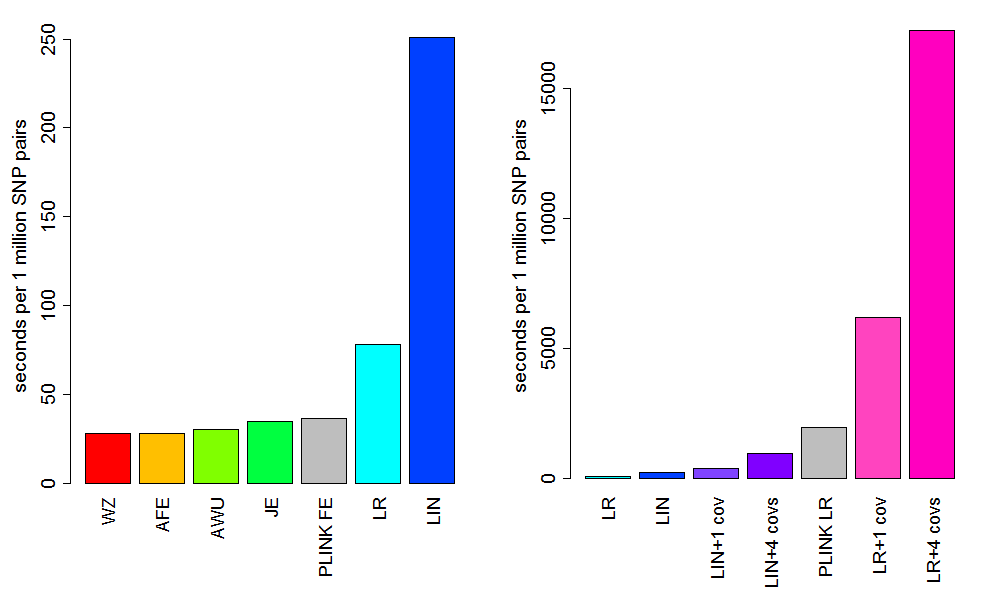
\includegraphics[width=400pt]{runtimesCASSI2.png}}
\caption{Runtimes to calculate 1 million SNP pair tests for the different tests in CASSI, plus two tests from PLINK, based on 4,498,500 SNP pair calculations of all the SNP pairs between 3000 SNPs with 1000 cases and 1000 controls (using a threshold of 0.0001 to output results). The tests left to right are: Wellek Ziegler (WZ); adjusted fast epistatis (AFE); adjusted Wu (AWU); joint effects (JE); PLINK fast epistasis (PLINK FE); logistic regression (LR); linear regression (LIN); linear regression with 1 and 4 covariates (LIN+1 cov and LIN+4 covs); PLINK logistic regression (PLINK LR); logistic regression with 1 and 4 covariates (LR+1 cov and LR+4 covs). Timings are based on the 64 bit Linux versions (machine: 6-Core AMD Opteron TM Processor with 2.6 GHz CPUs).}
\label{runtimes-fig}
\end{center}}
\end{figure}
}

%============ End of subsection "run-times"============


%================== End of section "multiple-tests"==================

\bibliographystyle{genepi}
\bibliography{/home/nrajh/work-other/tex/biblio}
\end{document}